% id: 131-03
% book: 개념원리 중학 3-2 · 13 상자그림
% section: 이런 문제가 시험에 나온다
% figure: crop:fig-131-03.png
% answer: ②, ④
% answer_source: 답지
% variant_level: 0 (원본 전사)
% 이 파일은 build.mjs 가 items.json 에서 만든다. 고칠 때는 items.json 을 고친다.
\smash{\raisebox{1.5mm}{\dmkichul{개념원리 중학 3-2 131쪽 03번}}}
\noindent\begin{minipage}[t]{0.58\linewidth}\vspace{0pt}\raggedright 오른쪽 그림은 연주네 반 학생들의 통학 시간을 조사하여 나타낸 상자그림이다. 다음 중 옳은 것을 모두 고르면? \mbox{(정답 2개)}\end{minipage}\hfill\begin{minipage}[t]{0.4\linewidth}\vspace{0pt}\centering \setlength{\dmfigw}{163.1pt}\ifdim\dmfigw>\linewidth\setlength{\dmfigw}{\linewidth}\fi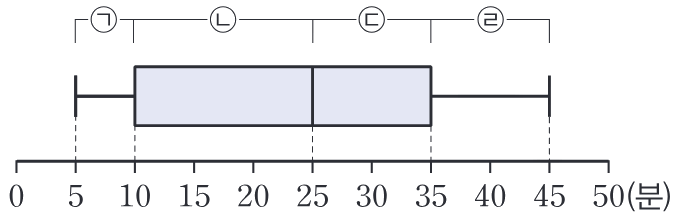
\includegraphics[width=\dmfigw]{figures/fig-131-03.png}\end{minipage}\par
\par\medskip\par\noindent\hangindent=1.4em\hangafter=1 {\small ①}\ 평균 통학 시간은 25분이다.\par\noindent\hangindent=1.4em\hangafter=1 {\small ②}\ 사분위수 범위는 25분이다.\par\noindent\hangindent=1.4em\hangafter=1 {\small ③}\ 통학 시간이 가장 긴 학생의 통학 시간은 35분이다.\par\noindent\hangindent=1.4em\hangafter=1 {\small ④}\ 통학 시간이 35분 이상인 학생은 전체의 약 $25\mkern3mu \%$이다.\par\noindent\hangindent=1.4em\hangafter=1 {\small ⑤}\ ㉠$\sim$㉣ 중 변량이 가장 흩어져 있는 구간은 ㉠이다.\par\medskip
